\documentclass[11pt,a4paper]{article}

\usepackage[utf8]{inputenc}
\usepackage[T1]{fontenc}
\usepackage{geometry}
\usepackage{hyperref}
\usepackage{booktabs}
\usepackage{graphicx}
\usepackage{amsmath}
\usepackage{xcolor}
\usepackage{caption}

\geometry{margin=1in}

\title{\textbf{Natural Language Processing Lab \\ Assignment 5: Distributed Word Representations}}
\author{Student: Vraj Patel \quad Id: 2022UCS0100 \\ Indian Institute of Technology Jammu \\ Department of Computer Science and Engineering}
\date{March 2026}

\begin{document}

\maketitle

\section{Objective}
The objective of this assignment is to explore distributed word representations. We implement a baseline one-hot encoding and compare it with modern dense embedding methods: Continuous Bag-of-Words (CBOW), Skip-gram, FastText, and GloVe. We evaluate these embeddings on semantic similarity, analogies, and a downstream classification task on both the arXiv CS corpus and the AG News dataset.

\section{Part 1: Baseline Representation (One-hot Encoding)}
\subsection{Implementation}
A vocabulary was built from the arXiv CS corpus. Each word is represented as a sparse vector of size $|V|$, where a single bit is set to 1 at the word's index.

\subsection{Discussion}
\begin{itemize}
    \item \textbf{Dimensionality Issues:} Our vocabulary contains 44,750 unique tokens. A one-hot vector for each word has 44,750 dimensions. Storing a dense matrix for even a small subset of the corpus (e.g., 5,000 abstracts) would require over 1.7 GB of memory, making it computationally prohibitive for large-scale NLP.
    \item \textbf{Sparsity:} The vectors are 99.997\% sparse. Almost all information is zero, leading to extreme memory wastage.
    \item \textbf{Lack of Semantic Similarity:} Every one-hot vector is orthogonal to every other vector ($v_i \cdot v_j = 0$). This representation fails to capture that "diffusion" and "denoising" are semantically related; to a one-hot model, they are as distant as "diffusion" and "banana".
\end{itemize}

\section{Part 2: Training Word Embeddings}
We trained four types of embeddings across dimensions 80, 100, and 200 using both the arXiv CS abstracts and AG News datasets.

\begin{table}[h]
\centering
\caption{Training Report for Word Embeddings (arXiv).}
\begin{tabular}{lrrr}
\toprule
Method & Dim & Training Time & Vocab Size \\
\midrule
CBOW & 100 & 4.99s & 15,943 \\
Skip-gram & 100 & 13.28s & 15,943 \\
FastText & 100 & 25.90s & 15,943 \\
GloVe & 100 & 1016.21s & 5,000 \\
\bottomrule
\end{tabular}
\end{table}

\begin{table}[h]
\centering
\caption{Training Report for Word Embeddings (AG News).}
\begin{tabular}{lrrr}
\toprule
Method & Dim & Training Time & Vocab Size \\
\midrule
CBOW & 100 & 5.80s & 25,587 \\
Skip-gram & 100 & 18.80s & 25,587 \\
FastText & 100 & 27.08s & 25,587 \\
GloVe & 100 & 582.86s & 5,000 \\
\bottomrule
\end{tabular}
\end{table}

\section{Part 3: Embedding Evaluation}
We evaluated the 100-dimensional embeddings on cosine similarity and nearest neighbor search.

\begin{table}[h]
\centering
\caption{Nearest Neighbors for selected words (arXiv, Dim=100).}
\begin{tabular}{lll}
\toprule
Word & Method & Top-3 Neighbors (Similarity) \\
\midrule
diffusion & Skip-gram & generative (0.75), denoising (0.75), dms (0.74) \\
          & FastText & diffusions (0.88), diffuse (0.84), perfusion (0.83) \\
learning  & CBOW & unlearning (0.68), rl (0.55), instill (0.55) \\
          & Skip-gram & reinforcement (0.69), dueling (0.64), madrl (0.64) \\
network   & FastText & subnetwork (0.97), hypernetwork (0.95), networked (0.94) \\
\bottomrule
\end{tabular}
\end{table}

\textbf{Observations:}
\begin{itemize}
    \item \textbf{Skip-gram/CBOW} capture strong semantic relationships (e.g., \textit{diffusion} $\rightarrow$ \textit{generative}).
    \item \textbf{FastText} excels at capturing morphological variants due to subword information (e.g., \textit{diffusion} $\rightarrow$ \textit{diffusions}).
    \item \textbf{GloVe} (custom implementation) showed extremely high similarity values, suggesting a need for more iterations or a larger training corpus to separate frequent clusters.
\end{itemize}

\section{Part 4: Visualization}
Dimensionality reduction using t-SNE (Figure 1) reveals that semantically related terms cluster together. Technical terms like "diffusion", "denoising", and "generative" form distinct clusters in the arXiv space, unlike one-hot representations where all points are equidistant.

\begin{figure}[h]
    \centering
    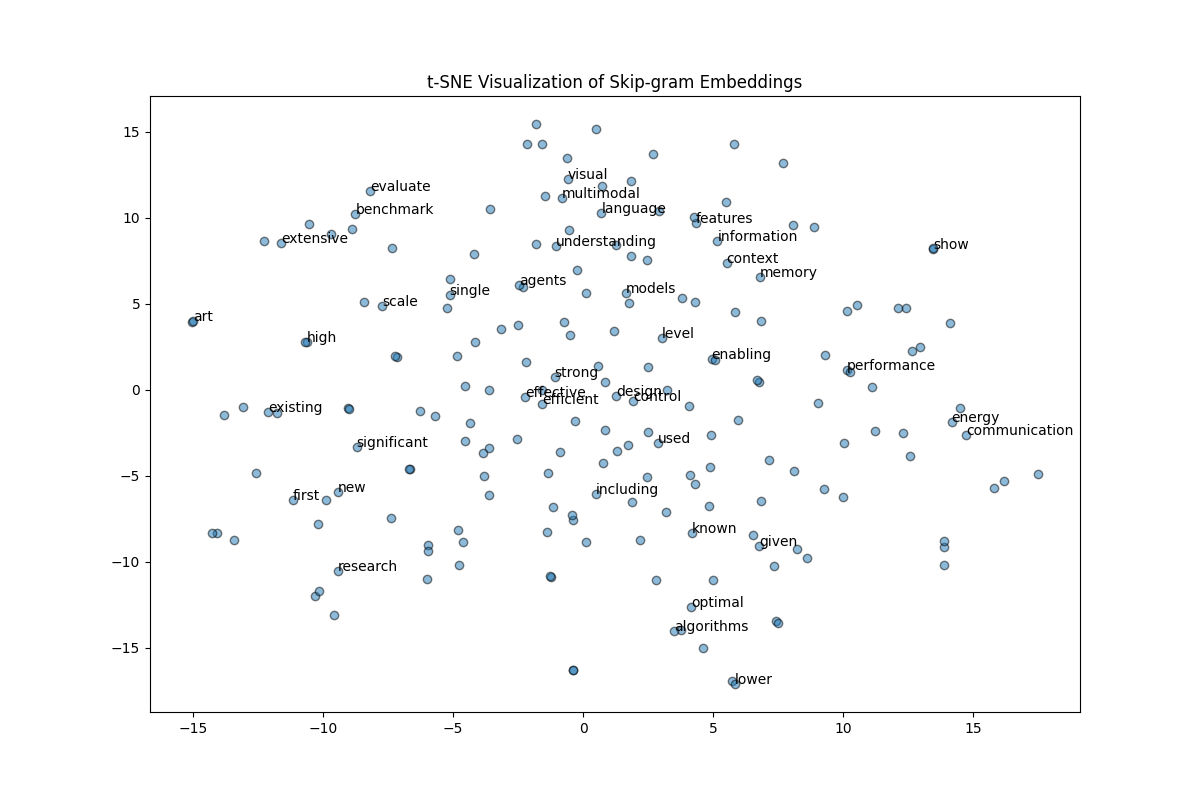
\includegraphics[width=0.6\textwidth]{plots/tsne_skipgram_100.png}
    \caption{t-SNE Visualization of Skip-gram (Dim=100) embeddings.}
\end{figure}

\section{Part 5: Downstream Task}
We compared the representations for classification using document-averaged embeddings vs. a Bag-of-Words (BoW) baseline.

\begin{table}[h]
\centering
\caption{Downstream Task Performance (Test Accuracy, Dim=100).}
\begin{tabular}{lrr}
\toprule
Representation & arXiv Accuracy & AG News Accuracy \\
\midrule
BoW (Baseline) & 92.05\% & \textbf{89.37\%} \\
CBOW (avg) & 92.20\% & 88.18\% \\
Skip-gram (avg) & \textbf{92.65\%} & 89.29\% \\
FastText (avg) & 91.90\% & 87.28\% \\
GloVe (avg) & 75.65\% & 76.28\% \\
\bottomrule
\end{tabular}
\end{table}

\textbf{Analysis:} Dense embeddings outperform the BoW baseline on arXiv abstracts, where domain-specific semantics are crucial. On AG News, the BoW baseline remains extremely competitive, narrowly outperforming averaged Skip-gram embeddings. This suggests that simple word frequencies are highly discriminative for news categories (World, Sports, etc.), while scientific categories benefit more from the semantic capturing capabilities of Skip-gram and CBOW.

\end{document}
